\documentclass[../main.tex]{subfiles}
\begin{document}



\chapter{Optimization}
\label{cha:cha_7}
\begin{center}
\Large{\textbf{CHAPTER OBJECTIVES}}
\end{center}

The primary objective of this chapter is to introduce you to how optimization can be
used to determine minima and maxima of both one-dimensional and multidimensional
functions. Specific objectives and topics covered are
\begin{itemize}
\item Understanding why and where optimization occurs in engineering and scientific
problem solving.
\item Recognizing the difference between one-dimensional and multidimensional
optimization.
\item Distinguishing between global and local optima.
\item Knowing how to recast a maximization problem so that it can be solved with a
minimizing algorithm.
\item Being able to define the golden ratio and understand why it makes onedimensional
optimization efficient.
\item Locating the optimum of a single-variable function with the golden-section search.
\item Locating the optimum of a single-variable function with parabolic interpolation.
\item Knowing how to apply the \texttt{fminbnd} function to determine the minimum of a
one-dimensional function.
\item Being able to develop MATLAB contour and surface plots to visualize twodimensional
functions.
\item Knowing how to apply the \texttt{fminsearch} function to determine the minimum of a
multidimensional function.

\end{itemize}

\newpage

\Large\color{cyan}{YOU’VE GOT A PROBLEM}

\smallskip
\color{black}
\normalsize{An object like a bungee jumper can be projected upward at a specified velocity. If it
is subject to linear drag, its altitude as a function of time can be computed as}
\smallskip
\begin{center}
\large{$\ z=z_0+\dfrac{m}{c}(v_0+\dfrac{mg}{c})(1-e^{-(c/m)t})-\dfrac{mg}{c}t$} \hfill {(7.1)}
\normalsize
\end{center}
\begin{figure}[H]
	\centering
	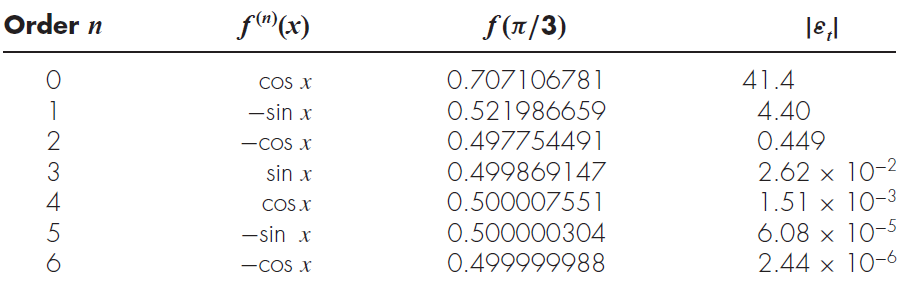
\includegraphics[width=0.75\linewidth]{fig_7_1}
	\caption{\textsf{Elevation as a function of time for an object initially projected upward with an initial velocity.}}
	\color{cyan} \rule{\linewidth}{0,5mm}
	\label{fig:fig_7_1}
\end{figure}
where $z$ = altitude (m) above the earth's surface (defined as $z$ = 0), $z_0$ = the initial altitude
(m), $m$ = mass (kg), $c$ = a linear drag coefficient (kg/s), $v_0$ = initial velocity (m/s), and $t$ =
time (s). Note that for this formulation, positive velocity is considered to be in the upward
direction. Given the following parameter values: $g = 9.81 m/s^2$, $z_0$ = 100 m, $v_0$ = 55 m/s,
$m$ = 80 kg, and $c$ = 15 kg/s, Eq. (7.1) can be used to calculate the jumper's altitude. As
displayed in Fig. 7.1, the jumper rises to a peak elevation of about 190 m at about $t$ = 4 s.
Suppose that you are given the job of determining the exact time of the peak elevation.
The determination of such extreme values is referred to as optimization. This chapter will
introduce you to how the computer is used to make such determinations.\bigskip

\section{A SIMPLE MATHEMATICAL MODEL}
\label{sec:sec_7_1}

In the most general sense, optimization is the process of creating something that is as
effective as possible. As engineers, we must continuously design devices and products that
perform tasks in an efficient fashion for the least cost. Thus, engineers are always confronting
optimization problems that attempt to balance performance and limitations. In
addition, scientists have interest in optimal phenomena ranging from the peak elevation of
projectiles to the minimum free energy.

From a mathematical perspective, optimization deals with finding the maxima and
minima of a function that depends on one or more variables. The goal is to determine the
values of the variables that yield maxima or minima for the function. These can then be
substituted back into the function to compute its optimal values.

Although these solutions can sometimes be obtained analytically, most practical
optimization problems require numerical, computer solutions. From a numerical standpoint,
optimization is similar in spirit to the root-location methods we just covered in
Chaps. 5 and 6. That is, both involve guessing and searching for a point on a function. The
fundamental difference between the two types of problems is illustrated in Fig. 7.2. Root
location involves searching for the location where the function equals zero. In contrast,
optimization involves searching for the function's extreme points.

\begin{figure}[H]
	\centering
	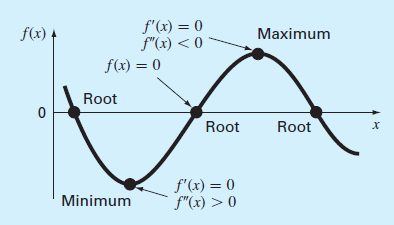
\includegraphics[width=0.5\linewidth]{fig_7_2}
	\caption{\textsf{A function of a single variable illustrating the difference between roots and optima.}}
	\color{cyan} \rule{\linewidth}{0,5mm}
	\label{fig:fig_7_2}
\end{figure}

As can be seen in Fig. 7.2, the optimums are the points where the curve is flat. In mathematical
terms, this corresponds to the x value where the derivative $f'(x)$ is equal to zero. Additionally, the second derivative,
$f''(x)$, indicates whether the optimum is a minimum or a maximum: if $f''(x) > 0$, 
the point is a maximum; if $f''(x) > 0$, the point is a minimum.

Now, understanding the relationship between roots and optima would suggest a possible
strategy for finding the latter. That is, you can differentiate the function and locate the
root (i.e., the zero) of the new function. In fact, some optimization methods do just this by
solving the root problem: $f''(x)$ = 0.
\newline
\color{cyan}\rule{\linewidth}{1mm}
\begin{exmp}
	\color{cyan}{Determining the Optimum Analytically by Root Location}
	\color{black}
	\smallskip
	
	\noindent Problem Statement:
	Determine the time and magnitude of the peak elevation based on
	Eq. (7.1). Use the following parameter values for your calculation: $g = 9.81 m/s^2$,
	z0 = 100 m, v0 = 55 m/s, m = 80 kg, and c = 15 kg/s.

	\noindent Solution: Equation (7.1) can be differentiated to give.
	\medskip

	$\dfrac{dz}{dt}=v_0e^{-(c/m)t}-\dfrac{mg}{c}(1-e^{-(c/m)t})$
	\medskip

	\noindent Note that because $v = dz/dt$, this is actually the equation for the velocity. The maximum
	elevation occurs at the value of t that drives this equation to zero. Thus, the problem
	amounts to determining the root. For this case, this can be accomplished by setting the derivative
	to zero and solving Eq. (E7.1.1) analytically for
	\medskip

	$t = \dfrac{m}{c}ln(1+\dfrac{cv_0}{mg})$
	\medskip

	\noindent Substituting the parameters gives
	\medskip

	$t=\dfrac{80}{15}ln(1+\dfrac{15(55)}{80(9.81)})=3.83166s$
	\medskip

	\noindent This value along with the parameters can then be substituted into Eq. (7.1) to compute the
	maximum elevation as
	\medskip

	\noindent $z=100+\dfrac{80}{15}(50+\dfrac{80(9.81)}{15})(1-e^{-(15/80)3.83166})-\dfrac{80(9.81)}{15}(3.83166)=192.8609m$                      
	\medskip

	We can verify that the result is a maximum by differentiating Eq. (E7.1.1) to obtain the
	second derivative
	\medskip

	$\dfrac{d^2z}{dt^2}=-\dfrac{c}{m}v_0e^{-(c/m)t}-ge^{-(c/m)t}=-9.81\dfrac{m}{s^2} $
	\medskip

	\noindent The fact that the second derivative is negative tells us that we have a maximum. Further,
	the result makes physical sense since the acceleration should be solely equal to the force of
	gravity at the maximum when the vertical velocity (and hence drag) is zero.

	Although an analytical solution was possible for this case, we could have obtained the
	same result using the root-location methods described in Chaps. 5 and 6. This will be left
	as a homework exercise.
	\newline
	\color{cyan}\rule{\linewidth}{1mm}
\end{exmp}

\color{black}

Although it is certainly possible to approach optimization as a roots problem, a variety
of direct numerical optimization methods are available. These methods are available for both
one-dimensional and multidimensional problems. As the name implies, one-dimensional
problems involve functions that depend on a single dependent variable. As in Fig. 7.3a, the
search then consists of climbing or descending one-dimensional peaks and valleys. Multidimensional
problems involve functions that depend on two or more dependent variables.

\begin{figure}[H]
	\centering
	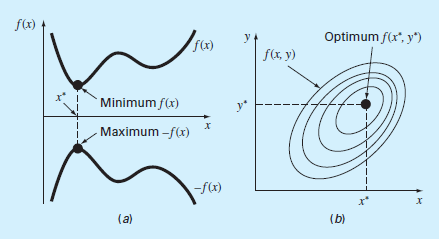
\includegraphics[width=0.5\linewidth]{fig_7_3}
	\caption{\textsf{(a) One-dimensional optimization. This figure also illustrates how minimization of $f(x)$ is
	equivalent to the maximization of $-f(x)$. (b) Two-dimensional optimization. Note that this
	figure can be taken to represent either a maximization (contours increase in elevation up to
	the maximum like a mountain) or a minimization (contours decrease in elevation down to the
	minimum like a valley).}}
	\color{cyan} \rule{\linewidth}{0,5mm}
	\label{fig:fig_7_3}
\end{figure}

In the same spirit, a two-dimensional optimization can again be visualized as searching out
peaks and valleys (Fig. 7.3b). However, just as in real hiking, we are not constrained to walk
a single direction; instead the topography is examined to efficiently reach the goal.

Finally, the process of finding a maximum versus finding a minimum is essentially
identical because the same value $x*$ both minimizes $f(x)$ and maximizes $-f(x)$. This
equivalence is illustrated graphically for a one-dimensional function in Fig. 7.3a.

In the next section, we will describe some of the more common approaches for onedimensional
optimization. Then we will provide a brief description of how MATLAB can
be employed to determine optima for multidimensional functions.\bigskip


\section{ONE-DIMENSIONAL OPTIMIZATION}
\label{sec:sec_7_2}

This section will describe techniques to find the minimum or maximum of a function of a
single variable $f(x)$. A useful image in this regard is the one-dimensional ''roller
coaster'' -like function depicted in Fig. 7.4. Recall from Chaps. 5 and 6 that root location
was complicated by the fact that several roots can occur for a single function. Similarly,
both local and global optima can occur in optimization.

A \textit{global optimum} represents the very best solution. A \textit{local optimum}, though not the
very best, is better than its immediate neighbors. Cases that include local optima are called
\textit{multimodal}. In such cases, we will almost always be interested in finding the global optimum.
In addition, we must be concerned about mistaking a local result for the global optimum.

Just as in root location, optimization in one dimension can be divided into bracketing
and open methods. As described in the next section, the golden-section search is an example
of a bracketing method that is very similar in spirit to the bisection method for root location.
This is followed by a somewhat more sophisticated bracketing approach-parabolic interpolation.
We will then show how these two methods are combined and implemented with
MATLAB's \texttt{fminbnd} function.

\begin{figure}[H]
	\centering
	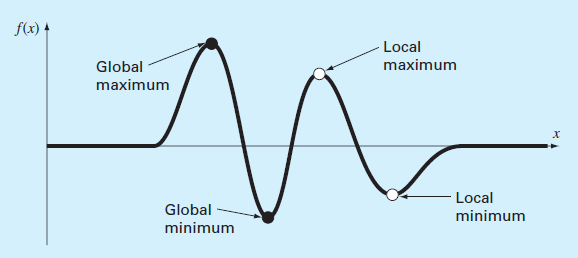
\includegraphics[width=0.75\linewidth]{fig_7_4}
	\caption{\textsf{(a) A function that asymptotically approaches zero at plus and minus $\infty$ and has two maximum and
	two minimum points in the vicinity of the origin. The two points to the right are local optima,
	whereas the two to the left are global.}}
	\color{cyan} \rule{\linewidth}{0,5mm}
	\label{fig:fig_7_4}
\end{figure}

\subsection{Golden-Section Search}

In many cultures, certain numbers are ascribed magical qualities. For example, we in theWest
are all familiar with ``lucky 7'' and ``Friday the 13th.'' Beyond such superstitious quantities,
there are several well-known numbers that have such interesting and powerful mathematical
properties that they could truly be called ``magical''. The most common of these are the ratio
of a circle's circumference to its diameter $\pi$ and the base of the natural logarithm $e$.

Although not as widely known, the golden ratio should surely be included in the pantheon
of remarkable numbers. This quantity, which is typically represented by the Greek
letter $\phi$ (pronounced: fee), was originally defined by Euclid (ca. 300 BCE) because of its
role in the construction of the pentagram or five-pointed star. As depicted in Fig. 7.5,
Euclid's definition reads: ``A straight line is said to have been cut in extreme and mean ratio
when, as the whole line is to the greater segment, so is the greater to the lesser.''

The actual value of the golden ratio can be derived by expressing Euclid's definition as
\medskip

$\dfrac{l_1+l_2}{l_1}=\dfrac{l_1}{l_2}$ \hfill {(7.2)}
\medskip

\noindent Multiplying by $l_1/l_2$ and collecting terms yields
\medskip

$\phi^2-\phi-1=0$ \hfill {(7.3)}
\medskip

\noindent where $\phi=l_1/l_2$. The positive root of this equation is the golden ratio:

$\phi = \dfrac{1+\sqrt{5}}{2}=1.61803398874989...$ \hfill {(7.4)}
\medskip

The golden ratio has long been considered aesthetically pleasing in Western cultures.
In addition, it arises in a variety of other contexts including biology. For our purposes, it
provides the basis for the golden-section search, a simple, general-purpose method for determining
the optimum of a single-variable function.

The golden-section search is similar in spirit to the bisection approach for locating
roots in Chap. 5. Recall that bisection hinged on defining an interval, specified by a lower
guess $(x_l)$ and an upper guess $(x_u)$ that bracketed a single root. The presence of a root between
these bounds was verified by determining that $f(x_l)$ and $f(x_u)$ had different signs.
The root was then estimated as the midpoint of this interval:
\medskip

$x_r=\dfrac{x_l+x_u}{2}$ \hfill {(7.5)}
\medskip

\begin{figure}[H]
	\centering
	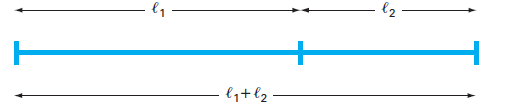
\includegraphics[width=0.65\linewidth]{fig_7_5}
	\caption{\textsf{Euclid's definition of the golden ratio is based on dividing a line into two segments so that the
	ratio of the whole line to the larger segment is equal to the ratio of the larger segment to the
	smaller segment. This ratio is called the golden ratio.}}
	\color{cyan} \rule{\linewidth}{0,5mm}
	\label{fig:fig_7_5}
\end{figure}

The final step in a bisection iteration involved determining a new smaller bracket. This was
done by replacing whichever of the bounds $x"_l$ or $x_u$ had a function value with the same sign
as $f(x_r)$. Akey advantage of this approach was that the new value $x_r$ replaced one of the old
bounds.

Now suppose that instead of a root, we were interested in determining the minimum of
a one-dimensional function. As with bisection, we can start by defining an interval that
contains a single answer. That is, the interval should contain a single minimum, and hence
is called \textit{unimodal}. We can adopt the same nomenclature as for bisection, where $x_l$ and $x_u$
defined the lower and upper bounds, respectively, of such an interval. However, in contrast
to bisection, we need a new strategy for finding a minimum within the interval. Rather than
using a single intermediate value (which is sufficient to detect a sign change, and hence a
zero), we would need two intermediate function values to detect whether a minimum
occurred.

The key to making this approach efficient is the wise choice of the intermediate points.
As in bisection, the goal is to minimize function evaluations by replacing old values with
new values. For bisection, this was accomplished by choosing the midpoint. For the
golden-section search, the two intermediate points are chosen according to the golden
ratio:
\smallskip

$x_1=x_l+d$ \hfill {(7.6)}

\smallskip
$x_2=x_u-d$ \hfill {(7.7)}

\noindent where
\smallskip

$d=(\phi-1)(x_u-x_l)$ \hfill {(7.8)}
\smallskip

\noindent The function is evaluated at these two interior points. Two results can occur:
\begin{enumerate}
	\item If, as in Fig. 7.6a, $f(x_1)<f(x_2)$, then $f(x_1)$ is the minimum, and the domain of $x$ to the
	left of $x_2$, from $x_l$ to $x_2$, can be eliminated because it does not contain the minimum. For
	this case, $x_2$ becomes the new $x_l$ for the next round.
	\item If $f(x_2)<f(x_1)$, then $f(x_2)$ is the minimum and the domain of $x$ to the right of $x_1$, from
	$x_1$ to $x_u$ would be eliminated. For this case, $x_1$ becomes the new $x_u$ for the next round.
\end{enumerate}

Now, here is the real benefit from the use of the golden ratio. Because the original $x_1$
and $x_2$ were chosen using the golden ratio, we do not have to recalculate all the function
values for the next iteration. For example, for the case illustrated in Fig. 7.6, the old $x_1$ becomes
the new $x_2$. This means that we already have the value for the new $f(x_2)$, since it is
the same as the function value at the old $x_1$.

To complete the algorithm, we need only determine the new $x_1$. This is done with
Eq. (7.6) with $d$ computed with Eq. (7.8) based on the new values of $x_l$ and $x_u$. A similar
approach would be used for the alternate case where the optimum fell in the left subinterval.
For this case, the new $x_2$ would be computed with Eq. (7.7).

As the iterations are repeated, the interval containing the extremum is reduced rapidly.
In fact, each round the interval is reduced by a factor of $\phi$ - 1(about 61.8\%). That means
that after 10 rounds, the interval is shrunk to about $0.618^{10}$ or 0.008 or 0.8\% of its initial
length. After 20 rounds, it is about 0.0066\%. This is not quite as good as the reduction
achieved with bisection (50\%), but this is a harder problem.

\begin{figure}[H]
	\centering
	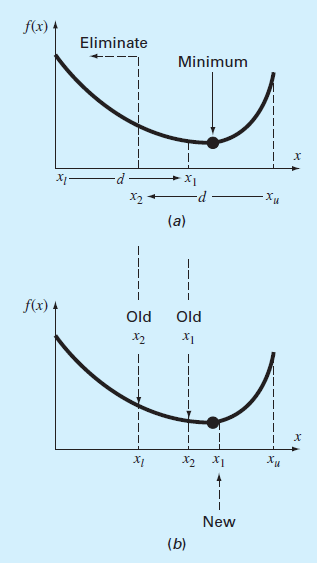
\includegraphics[width=0.4\linewidth]{fig_7_6}
	\caption{\textsf{(a) The initial step of the golden-section search algorithm involves choosing two interior points
	according to the golden ratio. (b) The second step involves defining a new interval that
	encompasses the optimum.}}
	\color{cyan} \rule{\linewidth}{0,5mm}
	\label{fig:fig_7_6}
\end{figure}


%\setcounter{exmp}{0} do resetowania licznika example

\begin{exmp}
	\color{cyan}{Golden-Section Search}
	\color{black}
	\smallskip
	
	\noindent Problem Statement:
	Use the golden-section search to find the minimum of

	$f(x)=\dfrac{x^2}{10}-2sin{x}$

	\noindent within the interval from $x_l=0$ to $x_u=4$

	\noindent Solution: First, the golden ratio is used to create the two interior points:
	\medskip

	$d = 0.61803(4 - 0) = 2.4721$
	\medskip

	$x_1 = 0 + 2.4721 = 2.4721$
	\medskip

	$x_2 = 4 - 2.4721 = 1.5279$
	\medskip

	\noindent The function can be evaluated at the interior points:
	\medskip

	$f(x_2) = \dfrac{1.5279^2}{10}-2sin(1.5279) = -1.7647)$
	\medskip

	$f(x_1) = \dfrac{2.4721^2}{10}-2sin(2.4721) = -0.6300)$
	\medskip

	Because $f(x_2)< f(x_1)$, our best estimate of the minimum at this point is that it is
	located at $x$ = 1.5279 with a value of $f(x) = -1.7647$. In addition, we also know that the
	minimum is in the interval defined by $x_l$, $x_2$, and $x_1$. Thus, for the next iteration, the lower
	bound remains $x_l = 0$, and $x_1$ becomes the upper bound, that is, $x_u = 2.4721$. In addition,
	the former $x_2$ value becomes the new $x_1$, that is, $x_1 = 1.5279$. In addition, we do not have to
	recalculate $f(x_1)$, it was determined on the previous iteration as $f(1.5279)=-1.7647$.

	All that remains is to use Eqs. (7.8) and (7.7) to compute the new value of $d$ and $x_2$:
	\medskip

	$d = 0.61803(2.4721 - 0) = 1.5279$
	\medskip

	$x_2 = 2.4721 - 1.5279 = 0.9443$

	\newpage
	The function evaluation at $x_2$ is $f(0.9943) = -1.5310$. Since this value is less than the
	function value at x1, the minimum is $f(1.5279) = -1.7647$, and it is in the interval prescribed
	by $x_2$, $x_1$, and $x_u$. The process can be repeated, with the results tabulated here:
	
	$$
	\begin{tabular}{|c|c|c|c|c|c|c|c|c|c|}
		\hline $i$ & $x_l$ & $f(x_l)$ & $x_2$ & $f(x_2)$ & $x_l$ & $f(x_l)$ & $x_u$ & $f(x_u)$ & $d$ \\
		\hline 1 & 0 & 0 & 1.5279 & -1.7647 & 2.4721 & -0.6300 & 4.0000 & 3.1136 & 2.4721 \\
		\hline 2 & 0 & 0 & 0.9443 & -1.5310 & 1.5279 & -1.7647 & 2.4721 & -0.6300 & 1.5279 \\
		\hline 3 & 0.9443 & -1.5310 & 1.5279 & -1.7647 & 1.8885 & -1.5432 & 2.4721 & -0.6300 & 0.9443 \\
		\hline 4 & 0.9443 & -1.5310 & 1.3050 & -1.7595 & 1.5279 & -1.7647 & 1.8885 & -1.5432 & 0.5836 \\
		\hline 5 & 1.3050 & -1.7595 & 1.5279 & -1.7647 & 1.6656 & -1.7136 & 1.8885 & -1.5432 & 0.3607 \\
		\hline 6 & 1.3050 & -1.7595 & 1.4427 & -1.7755 & 1.5279 & -1.7647 & 1.6656 & -1.7136 & 0.2229 \\
		\hline 7 & 1.3050 & -1.7595 & 1.3901 & -1.7742 & 1.4427 & -1.7755 & 1.5279 & -1.7647 & 0.1378 \\
		\hline 8 & 1.3901 & -1.7742 & 1.4427 & -1.7755 & 1.4752 & -1.7732 & 1.5279 & -1.7647 & 0.0851 \\
		\hline
	\end{tabular}
	$$
	
	\color{black} Note that the current minimum is highlighted for every iteration. After the eighth
	iteration, the minimum occurs at $x$ = 1.4427 with a function value of -1.7755. Thus, the
	result is converging on the true value of -1.7757 at $x$ = 1.4276.
	\newline
	\color{cyan}\rule{\linewidth}{1mm}
\end{exmp}

\color{black}
Recall that for bisection (Sec. 5.4), an exact upper bound for the error can be calculated
at each iteration. Using similar reasoning, an upper bound for golden-section search
can be derived as follows: Once an iteration is complete, the optimum will either fall in one
of two intervals. If the optimum function value is at $x_2$, it will be in the lower interval ($x_l,
x_2, x_1$). If the optimum function value is at $x_1$, it will be in the upper interval ($x_2, x_1, x_u$).
Because the interior points are symmetrical, either case can be used to define the error.

Looking at the upper interval ($x_2, x_1, x_u$), if the true value were at the far left, the maximum
distance from the estimate would be

$\Delta x_a = x_1 - x_2$
\medskip

$=x_l + (\phi - 1)(x_u - x_l ) - x_u + (\phi - 1)(x_u - x_l )$
\medskip

$=(x_l - x_u) + 2(\phi - 1)(x_u - x_l )$
\medskip

$=(2\phi - 3)(x_u - x_l )$
\medskip

\noindent or 0.2361 ($x_u - x_l$). If the true value were at the far right, the maximum distance from the
estimate would be

$\Delta x_b = x_u - x_1$
\medskip

$=x_u - x_l - (\phi - 1)(x_u - x_l )$
\medskip

$=(x_u - x_l) - (\phi - 1)(x_u - x_l )$
\medskip

$=(2 -\phi)(x_u - x_l)$
\medskip

\noindent or 0.3820 ($x_u - x_l$). Therefore, this case would represent the maximum error. This result can
then be normalized to the optimal value for that iteration $x_opt$ to yield

$\epsilon_a = (2 - \phi)|\dfrac{x_u-x_l}{x_{opt}}|\times 100\% $ \hfill {(7.9)}

\noindent This estimate provides a basis for terminating the iterations.

An M-file function for the golden-section search for minimization is presented in
Fig. 7.7. The function returns the location of the minimum, the value of the function, the
approximate error, and the number of iterations.

The M-file can be used to solve the problem from Example 7.1.

\begin{lstlisting}[numbers=none,frame=none]
	>> g=9.81;v0=55;m=80;c=15;z0=100;
	>> z=@(t) -(z0+m/c*(v0+m*g/c)*(1-exp(-c/m*t))-m*g/c*t);
	>> [xmin,fmin,ea,iter]=goldmin(z,0,8)

	xmin =
		3.8317
	fmin =
		-192.8609
	ea =
		6.9356e-005
\end{lstlisting}

\noindent Notice how because this is a maximization, we have entered the negative of Eq. (7.1).
Consequently, \texttt{fmin} corresponds to a maximum height of 192.8609.

You may be wondering why we have stressed the reduced function evaluations of the
golden-section search. Of course, for solving a single optimization, the speed savings
would be negligible. However, there are two important contexts where minimizing the
number of function evaluations can be important. These are
\begin{enumerate}
	\item Many evaluations. There are cases where the golden-section search algorithm may be a
	part of a much larger calculation. In such cases, it may be called many times. Therefore,
	keeping function evaluations to a minimum could pay great dividends for such cases.
	
	\begin{figure}[H]
		\centering
		
\includegraphics[width=0.0001\linewidth]{fig_7_7}
		\caption{\textsf{An M-file to determine the minimum of a function with the golden-section search.}}
		\color{cyan} \rule{\linewidth}{0,5mm}
		\label{fig:fig_7_7}
	\end{figure}

	\item Time-consuming evaluation. For pedagogical reasons, we use simple functions in
	most of our examples. You should understand that a function can be very complex
	and time-consuming to evaluate. For example, optimization can be used to estimate
	the parameters of a model consisting of a system of differential equations. For such
	cases, the ``function'' involves time-consuming model integration. Any method that
	minimizes such evaluations would be advantageous.
\end{enumerate}

\begin{figure}[H]
	\centering
	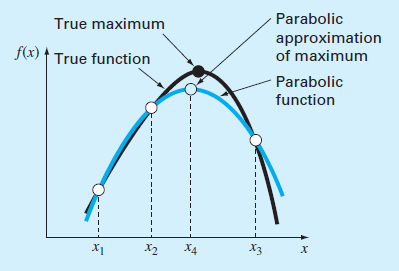
\includegraphics[width=0.5\linewidth]{fig_7_8}
	\caption{\textsf{Graphical depiction of parabolic interpolation.}}
	\color{cyan} \rule{\linewidth}{0,5mm}
	\label{fig:fig_7_8}
\end{figure}

\subsection{Parabolic Interpolation}

\noindent Parabolic interpolation takes advantage of the fact that a second-order polynomial often
provides a good approximation to the shape of f (x) near an optimum (Fig. 7.8).

Just as there is only one straight line connecting two points, there is only one parabola
connecting three points. Thus, if we have three points that jointly bracket an optimum, we
can fit a parabola to the points. Then we can differentiate it, set the result equal to zero, and
solve for an estimate of the optimal x. It can be shown through some algebraic manipulations
that the result is
\begin{lstlisting}[numbers=none,frame=none]
asdasdas
asdasd
asd
asd
as
dasd
asd
das
df
aag
\end{lstlisting}




\medskip

$x_4 = x_2 - \dfrac{1}{2}\dfrac{(x_2-x_1)^2[f(x_2)-f(x_3)]-(x_2-x_3)^2[f(x_2)-f(x_1)]}{(x_2-x_1)[f(x_2)-f(x_3)]-(x_2-x_3)[f(x_2)-f(x_1)]} $ \hfill {(7.10)}
\medskip

\noindent where $x1$, $x2$, and $x3$ are the initial guesses, and $x4$ is the value of $x$ that corresponds to the
optimum value of the parabolic fit to the guesses.

\end{document}